\begin{figure}
  \setlength{\unitlength}{\textwidth}
  \begin{picture}(1,0.25)
    % % %90
    \put(0.02,0.03){\includegraphics[width=0.3\unitlength]{../FnP/gnuplot/fsi_displacement.eps}}
    \put(0.36,0.03){\includegraphics[width=0.3\unitlength]{../FnP/gnuplot/fsi_velocity.eps}}
    \put(0.72,0.03){\includegraphics[width=0.3\unitlength]{../FnP/gnuplot/fsi_power.eps}}
    
    \put(0.03,0.17){$\frac{A}{D}$}
    \put(0.36,0.17){$\frac{V}{D}$}
    \put(0.68,0.17){$\frac{P_{m}}{\rho \mathcal{A}U^3 }$}
    
    \put(0.18,0.0){\ustar} 	
    \put(0.51,0.0){\ustar}
    \put(0.87,0.0){\ustar}

    \put(0.092,0.21){\small(a)}
    \put(0.42,0.21){\small(b)}
    \put(0.78,0.21){\small(c)}

  \end{picture}  

  \caption{Comparison of data generated using the quasi-static theory (\ding{83}) and full DNS simulations (\ding{108}). (a) Displacement amplitude, (b) velocity amplitude and (c) mean power as a function of \ustar. Data were obtained at $Re=165$ and $\zeta=0.075$. An average difference of $34\%$ is observed for both displacement and velocity amplitude. However, the essential physics i.e the rise and fall of mean power, is captured by DNS simulations.}
    \label{fig:FSI_QSS_compare}
\end{figure}